% !TEX program = pdflatex
% ---------------------------------------------------------------------------
% Slide deck — first structural draft, oriented on Outline.tex
% Minimal skeleton: one section per outline section, frames to be populated
% step by step. Figures live in Figures/, table fragments in Tables/.
% Style rule: no dashes, colons, or semicolons as sentence breaks in
% rendered text.
% ---------------------------------------------------------------------------
\documentclass[aspectratio=169,11pt]{beamer}

% --- Clean, low-color look ------------------------------------------------
\usetheme{default}
\setbeamertemplate{navigation symbols}{}
\setbeamertemplate{caption}{\insertcaption}
\setbeamersize{text margin left=1.6em, text margin right=1.6em}

\definecolor{ink}{RGB}{35,38,45}     % near-black text
\definecolor{slate}{RGB}{90,97,110}  % muted gray accent
\definecolor{faint}{RGB}{175,180,188}% light gray rules
\definecolor{wine}{RGB}{130,60,60}   % desaturated red for \alert only

\setbeamercolor{normal text}{fg=ink,bg=white}
\setbeamercolor{structure}{fg=ink}
\setbeamercolor{alerted text}{fg=wine}
\setbeamercolor{frametitle}{fg=ink,bg=white}
\setbeamercolor{title}{fg=ink}
\setbeamercolor{itemize item}{fg=slate}
\setbeamercolor{itemize subitem}{fg=slate}
\setbeamercolor{enumerate item}{fg=slate}
\setbeamercolor{section in toc}{fg=ink}
\setbeamercolor{page number in head/foot}{fg=slate}

\setbeamerfont{title}{series=\bfseries,size=\Large}
\setbeamerfont{frametitle}{series=\bfseries,size=\large}
\setbeamerfont{author}{size=\normalsize}
\setbeamerfont{date}{size=\small}
\setbeamerfont{framesubtitle}{size=\small}
\setbeamertemplate{itemize items}[circle]
\setbeamertemplate{footline}[frame number]

% Compact table of contents (default spacing overflows the Roadmap frame)
\setbeamerfont{section in toc}{size=\small}
\setbeamertemplate{section in toc}{%
  {\color{slate}\inserttocsectionnumber.}\hspace{0.5em}\inserttocsection\par}

% Beamer hard-codes \vskip1.5em between TOC section entries, outside any
% template — patch it down so the entries sit closer together.
\usepackage{etoolbox}
\makeatletter
\patchcmd{\beamer@sectionintoc}{\vskip1.5em}{\vskip0.5em}{}{}
\makeatother

% Frame title with an optional gray subtitle and a thin rule underneath
\setbeamertemplate{frametitle}{%
  \vskip1.2ex
  {\usebeamerfont{frametitle}\usebeamercolor[fg]{frametitle}\insertframetitle\strut\par}%
  \ifx\insertframesubtitle\empty\else
    {\usebeamerfont{framesubtitle}\color{slate}\insertframesubtitle\strut\par}%
  \fi
  \vskip0.4ex
  {\color{faint}\hrule height 0.4pt}%
  \vskip1.2ex
}

\usepackage{booktabs}
\usepackage{siunitx}   % needed by the estout table fragments (S columns)
\usepackage{graphicx}
\graphicspath{{Figures/}}

% Yellow marker for unresolved placeholders
\newcommand{\todohl}[1]{\colorbox{yellow!45}{\strut #1}}

% Light gray takeaway box
\definecolor{mist}{RGB}{242,243,246}
\setbeamercolor{takeawaybox}{bg=mist,fg=ink}
\newcommand{\takeaway}[1]{%
  \begin{beamercolorbox}[sep=0.6em,wd=\textwidth]{takeawaybox}
    \textbf{Takeaway.} #1
  \end{beamercolorbox}}

% Key point box leading each literature slide
\newcommand{\keypoint}[1]{%
  \begin{beamercolorbox}[sep=0.6em,wd=\textwidth]{takeawaybox}
    \textbf{Key point.} #1
  \end{beamercolorbox}}

% --- Title and authors as in main.tex --------------------------------------
\title{Hedge Funds Strategies}
\author{Felix Hermes \and Davide Tomio}
\date{\today}

\begin{document}

% ---------------------------------------------------------------------------
\begin{frame}
  \titlepage
\end{frame}

% ---------------------------------------------------------------------------
\begin{frame}{This paper}
  \begin{itemize}
    \item \textbf{Fact 1.} Hedge funds are the marginal intermediaries between sovereign cash and futures markets, and the trade they run is not the modeled basis trade.
    \item \textbf{Fact 2.} The trade concentrates in cheap off-the-run bonds and is duration neutral but convexity exposed.
    \item \textbf{Fact 3.} Three dealers finance more than half of it.
  \end{itemize}
\end{frame}

% ---------------------------------------------------------------------------
\begin{frame}{Roadmap}
  \tableofcontents[hideallsubsections]
\end{frame}



% ===========================================================================
\section{Data and setting}
\begin{frame}{Data and setting}
  \textbf{One dataset per leg of the trade}
  \begin{itemize}
    \item \textbf{Repo leg}\quad SFTDS transaction data
    \item \textbf{Futures leg}\quad EMIR transaction data
  \end{itemize}
  \bigskip
  \textbf{Coverage}
  \begin{itemize}
    \item SFTDS and EMIR report every transaction that involves at least one euro area established entity.
    \item Euro area dealers are global banks, so the data cover both parts of EUR and USD markets.
    \item US coverage is naturally thinner. A trade between two non euro area entities, for example a US dealer facing an offshore fund, never enters the data.
  \end{itemize}
\end{frame}

\begin{frame}{Data and setting}{Where the funds trading German futures sit}
  \begin{columns}[T]
    \begin{column}{.5\textwidth}\centering
      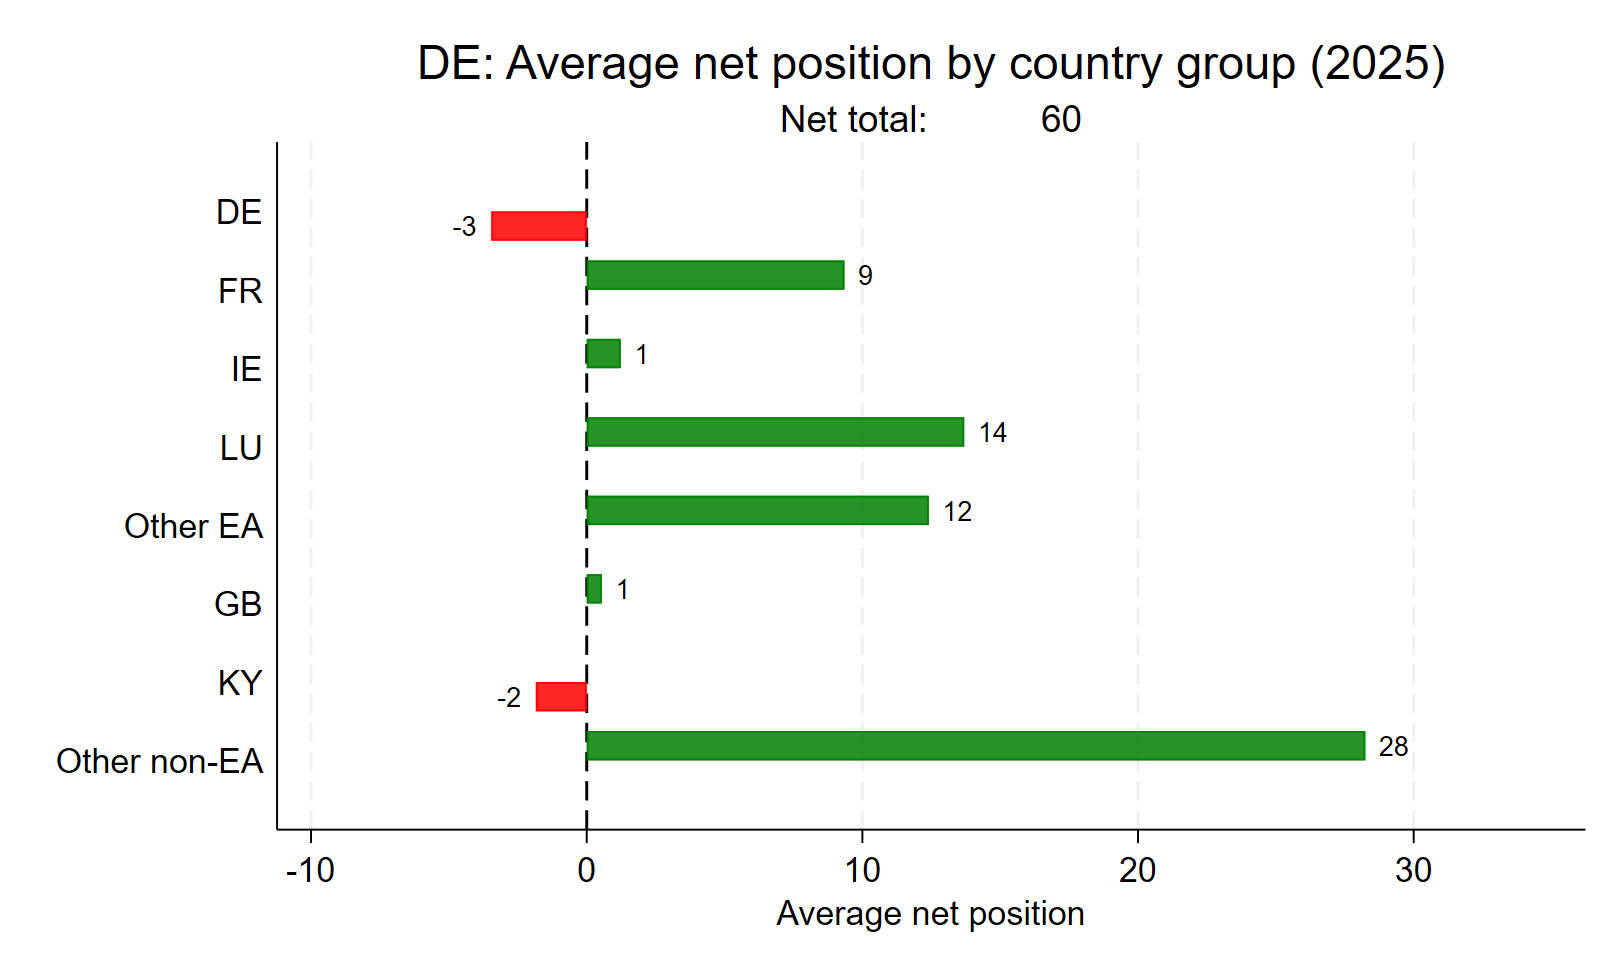
\includegraphics[width=\linewidth,height=.55\textheight,keepaspectratio]{DE_countries_2022.png}\\
      {\small\color{slate} 2021 and 2022}
    \end{column}
    \begin{column}{.5\textwidth}\centering
      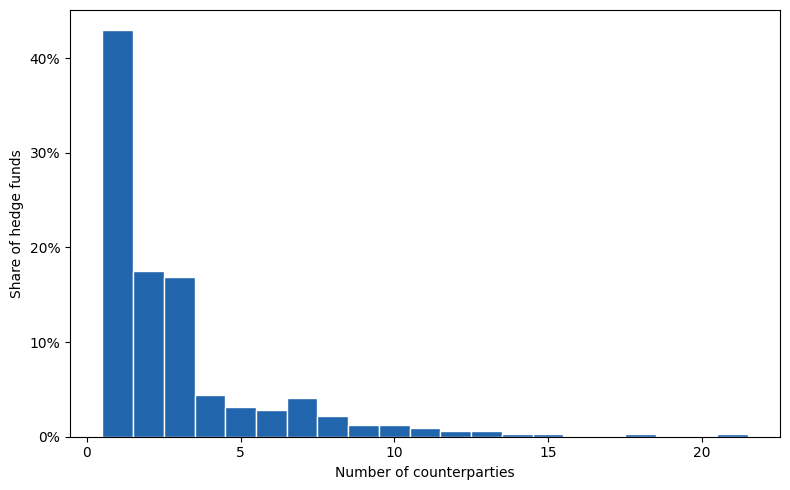
\includegraphics[width=\linewidth,height=.55\textheight,keepaspectratio]{DE_countries_2025.png}\\
      {\small\color{slate} 2025}
    \end{column}
  \end{columns}
  \medskip
  \centering
  {\small\color{slate} Average daily net position in Bund, Bobl, Schatz and Buxl futures by fund country, long minus short notional in billions of euro, summed within date and country group and averaged over the window}
\end{frame}

\begin{frame}{Data and setting}{Where the funds trading US futures sit}
  \begin{columns}[T]
    \begin{column}{.5\textwidth}\centering
      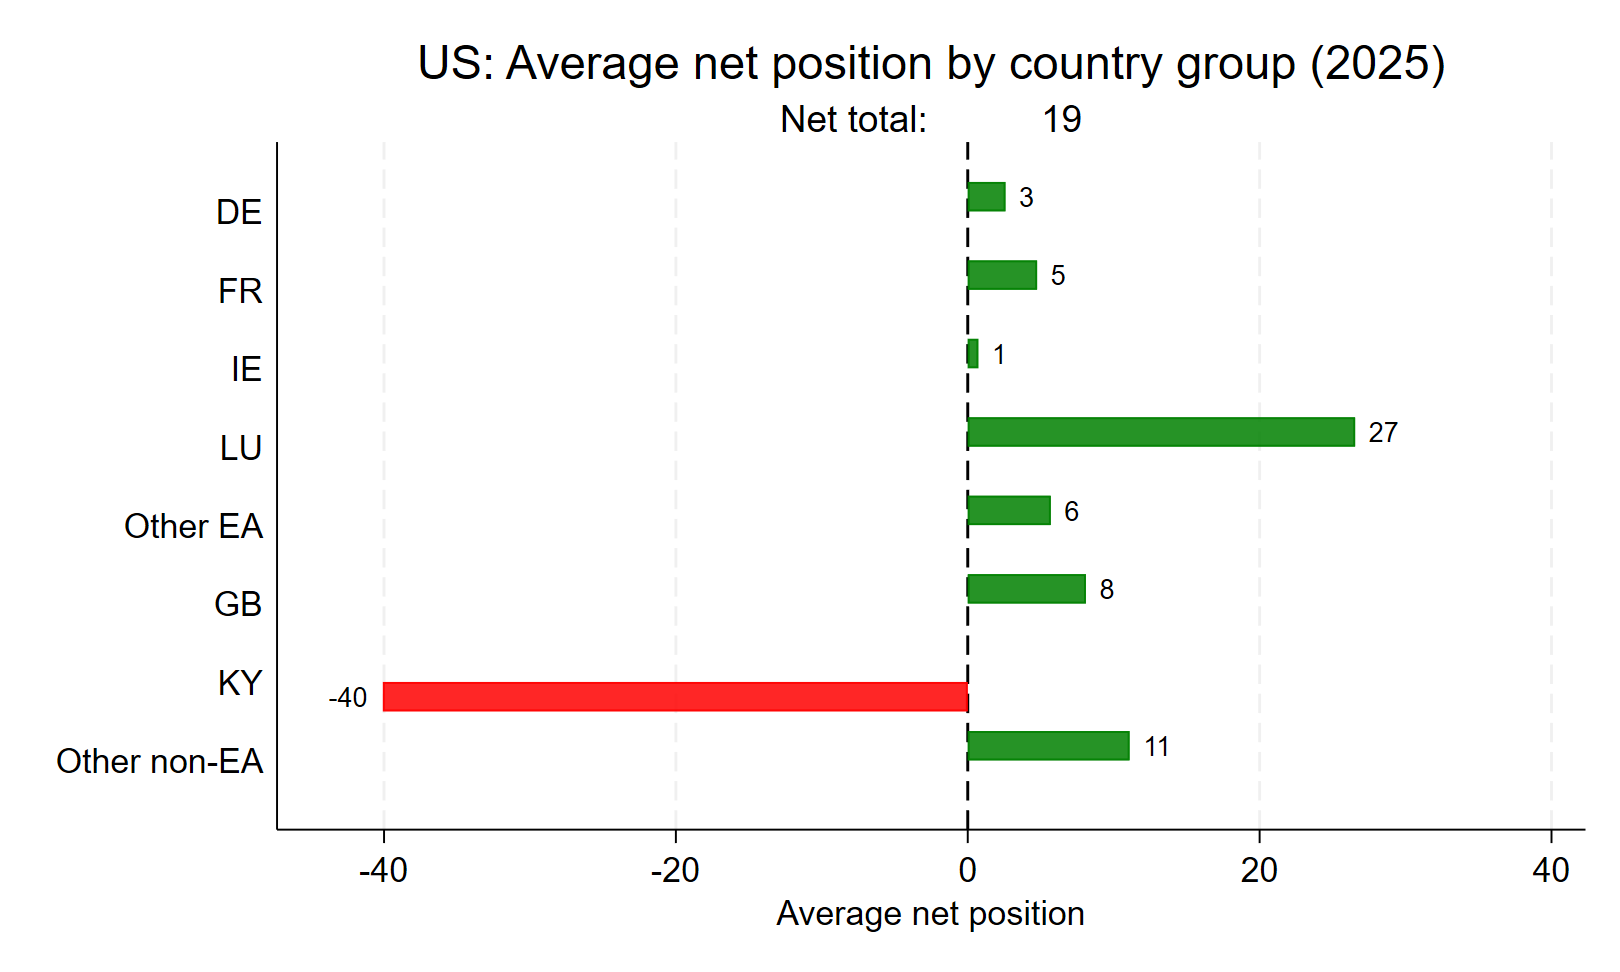
\includegraphics[width=\linewidth,height=.55\textheight,keepaspectratio]{US_countries_2022.png}\\
      {\small\color{slate} 2021 and 2022}
    \end{column}
    \begin{column}{.5\textwidth}\centering
      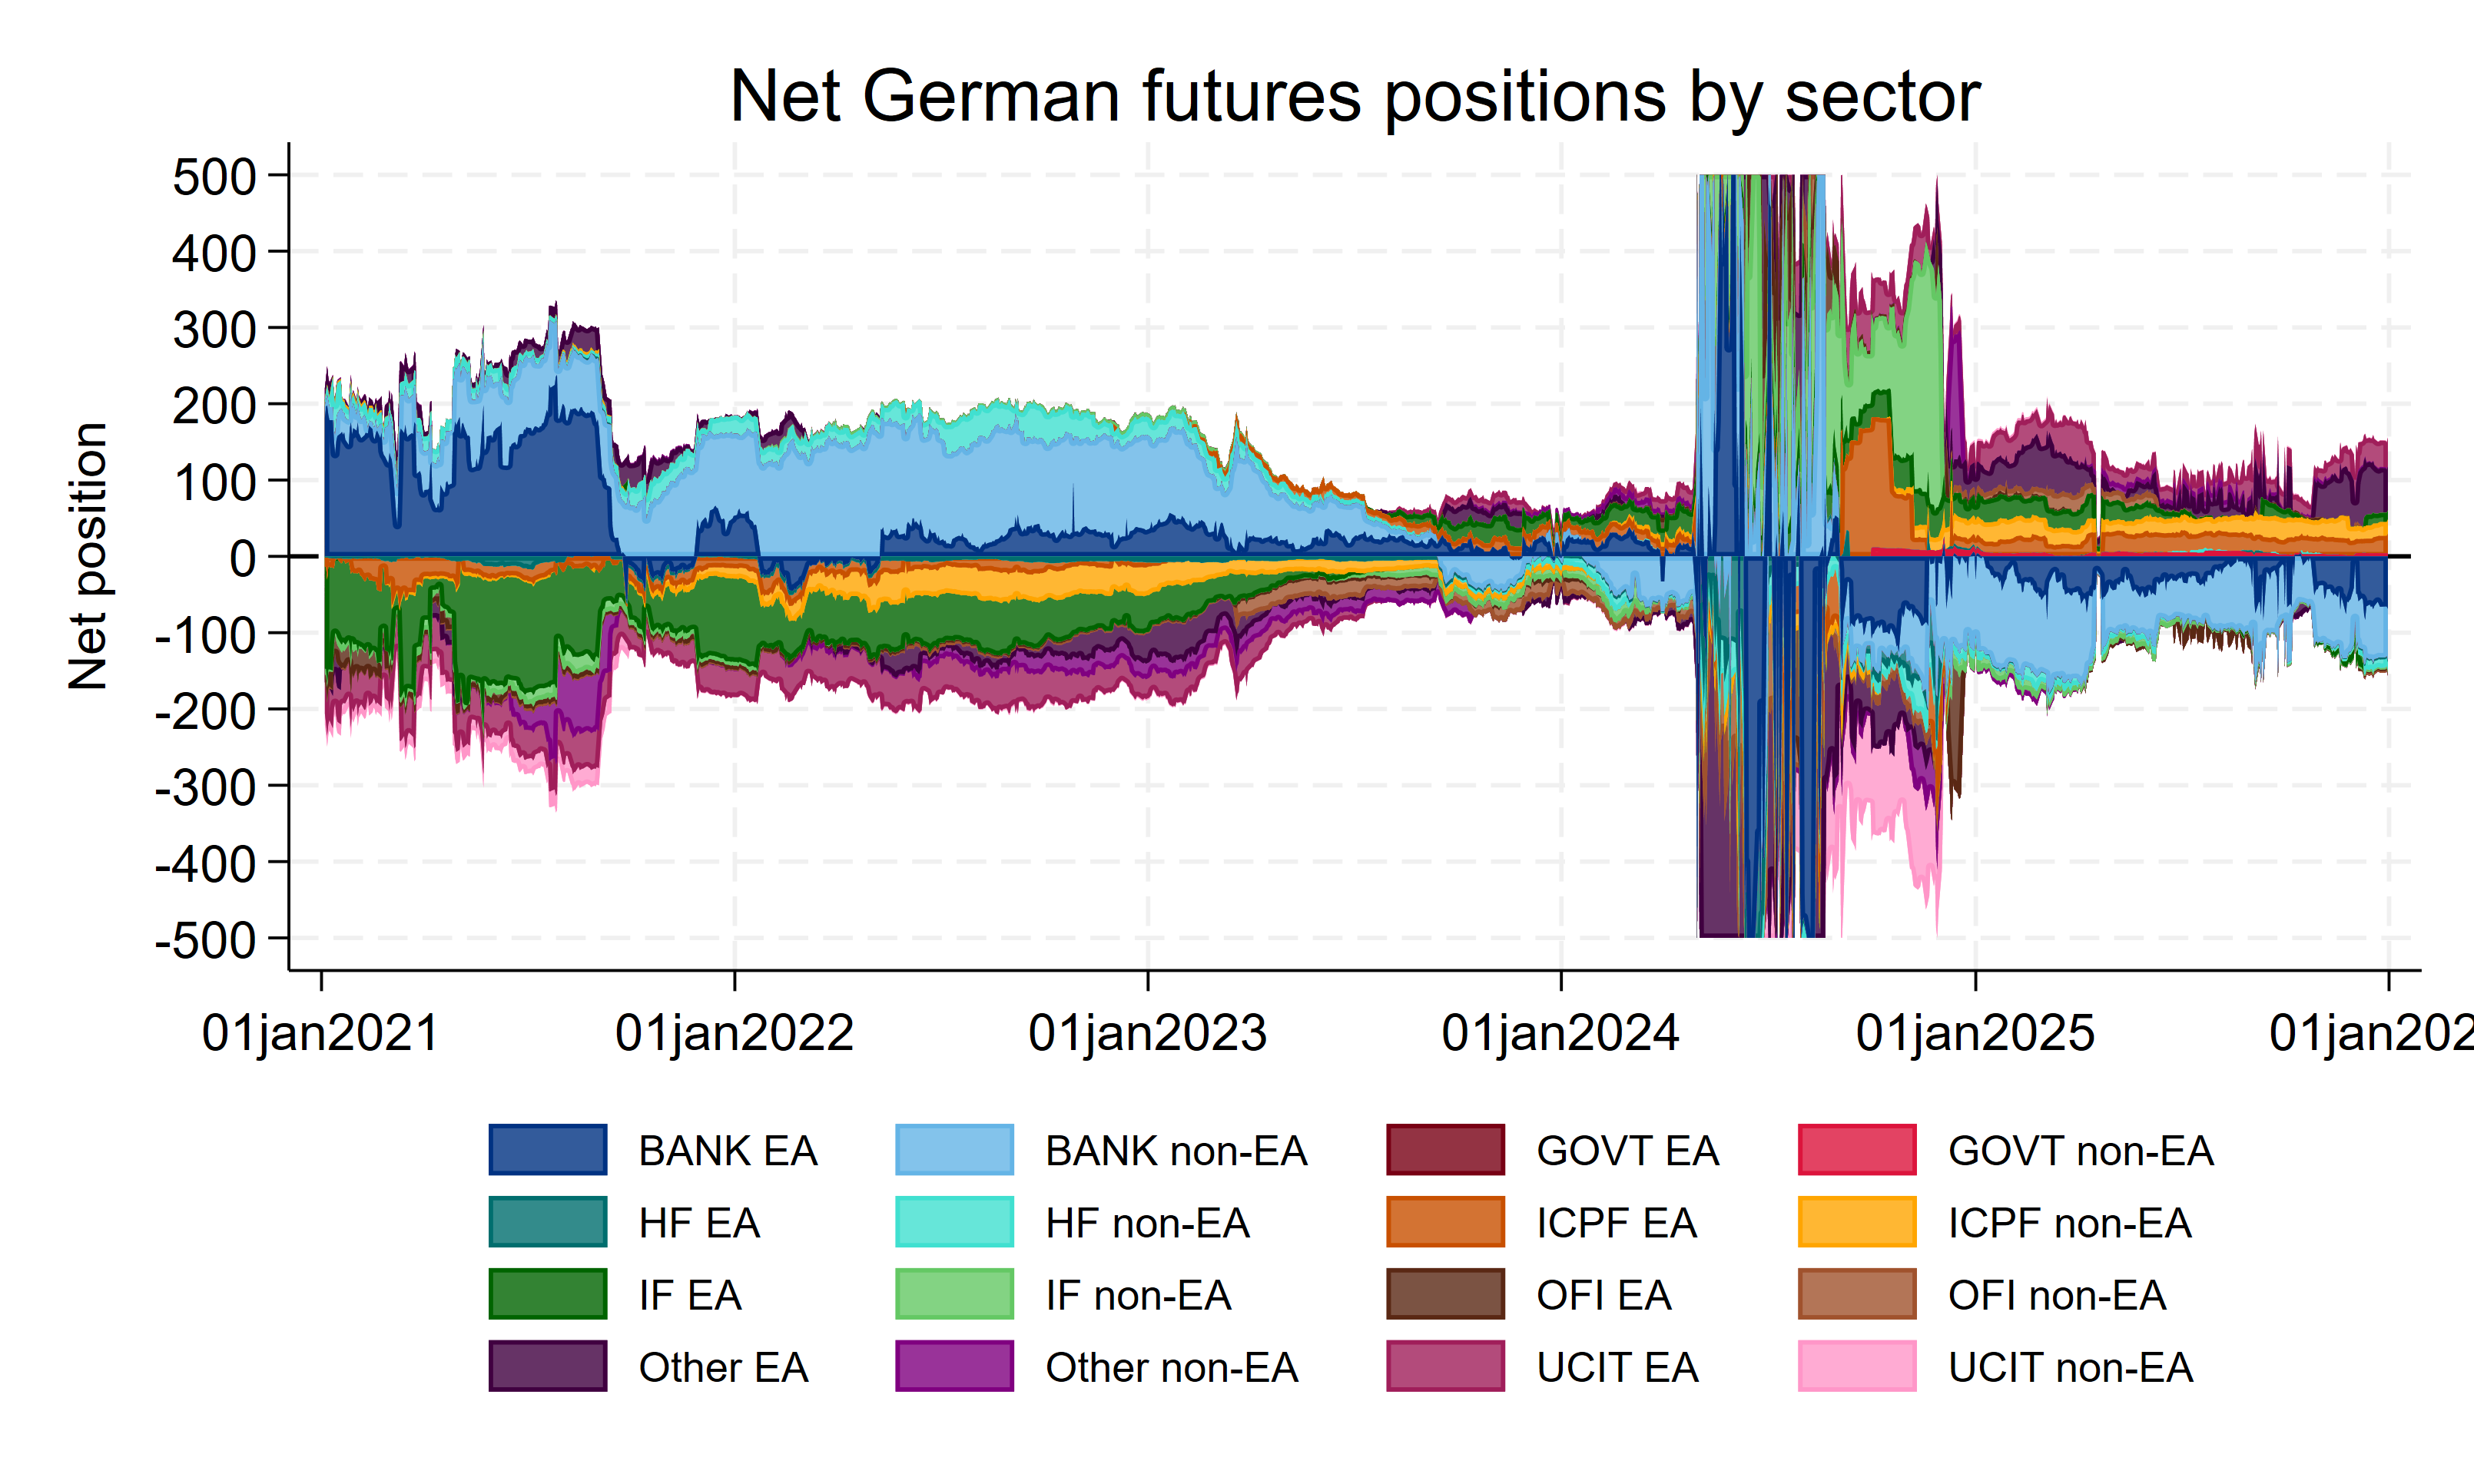
\includegraphics[width=\linewidth,height=.55\textheight,keepaspectratio]{US_countries_2025.png}\\
      {\small\color{slate} 2025}
    \end{column}
  \end{columns}
  \medskip
  \centering
  {\small\color{slate} Average daily net position in US Treasury futures by fund country, long minus short notional in billions of dollars, summed within date and country group and averaged over the window}
\end{frame}

\begin{frame}{Data and setting}{Net positions in German government bond futures}
  \centering
  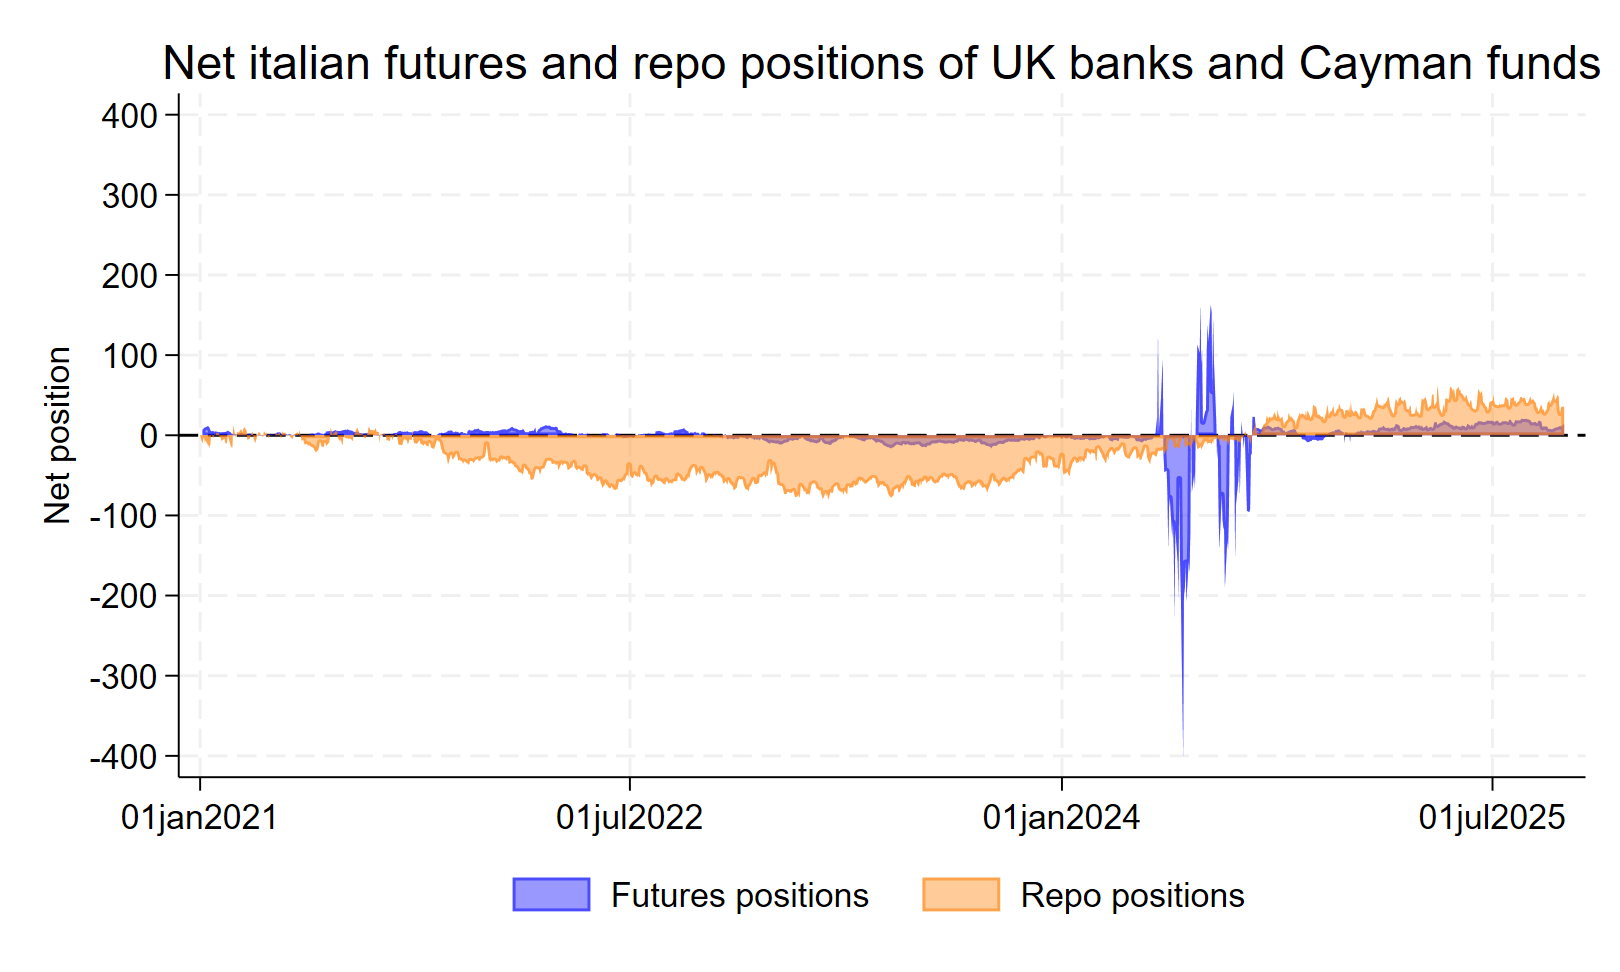
\includegraphics[width=.88\textwidth,height=.7\textheight,keepaspectratio]{net_repo_futures_DE.png}\\
  {\small\color{slate} Daily net futures and net repo positions of UK banks and Cayman funds in German government bonds, summed across entities and capped at plus and minus 400}
\end{frame}

\begin{frame}{Data and setting}{Hedge fund activity in EUR and USD repo markets}
  \vspace{-0.6em}
  \begin{center}\scriptsize
  \begin{tabular}{lrr}
    \toprule
    Share of gross volume (percent) & EUR & USD \\
    \midrule
    \multicolumn{3}{l}{\textit{Panel A. Hedge funds}} \\
    Funds active in both currencies & 99.3 & 98.3 \\
    Top 5 funds & 46.0 & 40.0 \\
    \midrule
    \multicolumn{3}{l}{\textit{Panel B. Counterparties}} \\
    Counterparties active in both currencies & 96.3 & 98.1 \\
    US primary dealers & 46.4 & 88.4 \\
    Funds using a single entity within a banking group & 87.2 & 98.2 \\
    \midrule
    \multicolumn{3}{l}{\textit{Panel C. Cross currency relationships}} \\
    Banking groups that are also counterparties in the other currency & 80.8 & 97.0 \\
    \quad \textit{of which} through the exact same entity within the banking group & 89.8 & 97.6 \\
    \bottomrule
  \end{tabular}
  \end{center}
  {\tiny\color{slate} Volume shares are the fraction of total gross nominal volume in each currency. A fund is active in both currencies if it appears at least once as borrower or lender in both EUR and USD repos over the sample period. Counterparties are matched to banking groups. The sample covers non centrally cleared specific collateral repos in government securities.\par}
\end{frame}

% ===========================================================================
\section{Measuring basis positions}
\begin{frame}{Measuring basis positions}
  \textbf{Three building blocks}
  \begin{itemize}
    \item \textbf{Bond day panel}\quad fitted yields, pricing errors, duration and convexity, with CTD, deliverable and on the run flags
    \item \textbf{Repo panel}\quad SFTDS positions by fund, bond and day
    \item \textbf{Futures panel}\quad EMIR positions by fund, contract and day, linked to bonds through the deliverable set
  \end{itemize}
  \smallskip
  The panels merge in any combination of fund, bond and date.
  \medskip

  \textbf{Classifying positions}
  \begin{itemize}
    \item A fund that is long the future and short the bond, or the reverse, runs a basis trade.
    \item Bond positions without an offsetting futures leg are directional.
  \end{itemize}
  \medskip
  \textbf{Validation}
  \begin{itemize}
    \item Compare positions and captured market share with the OFR hedge fund monitor.
  \end{itemize}
\end{frame}

% ===========================================================================
\section{Anatomy of the trade}
\begin{frame}{Anatomy of the trade}
  \begin{itemize}
    \item Positions are concentrated in a handful of funds.
    \item Five dealers finance more than half of the trade.
    \item The bonds are neither cheapest to deliver nor on the run and show positive pricing errors in both jurisdictions.
  \end{itemize}
  \bigskip
  \takeaway{Funds are paid to hold what curve sensitive investors and dealers do not want, providing liquidity and convergence in the illiquid segment.}
\end{frame}

\begin{frame}{Anatomy of the trade}{Net repo positions of hedge funds in sovereign bonds}
  \begin{columns}[T]
    \begin{column}{.5\textwidth}\centering
      \includegraphics[width=\linewidth,height=.55\textheight,keepaspectratio]{net_repo_US.png}\\
      {\small\color{slate} US}
    \end{column}
    \begin{column}{.5\textwidth}\centering
      \includegraphics[width=\linewidth,height=.55\textheight,keepaspectratio]{net_repo_EA.png}\\
      {\small\color{slate} Euro area}
    \end{column}
  \end{columns}
  \medskip
  \centering
  {\small\color{slate} Daily net repo position of hedge funds, borrowing minus lending volume summed across funds and bonds, in billions. The euro area panel splits the total by issuer}
\end{frame}

\begin{frame}{Anatomy of the trade}{Positions are concentrated in a handful of funds}
  \centering
  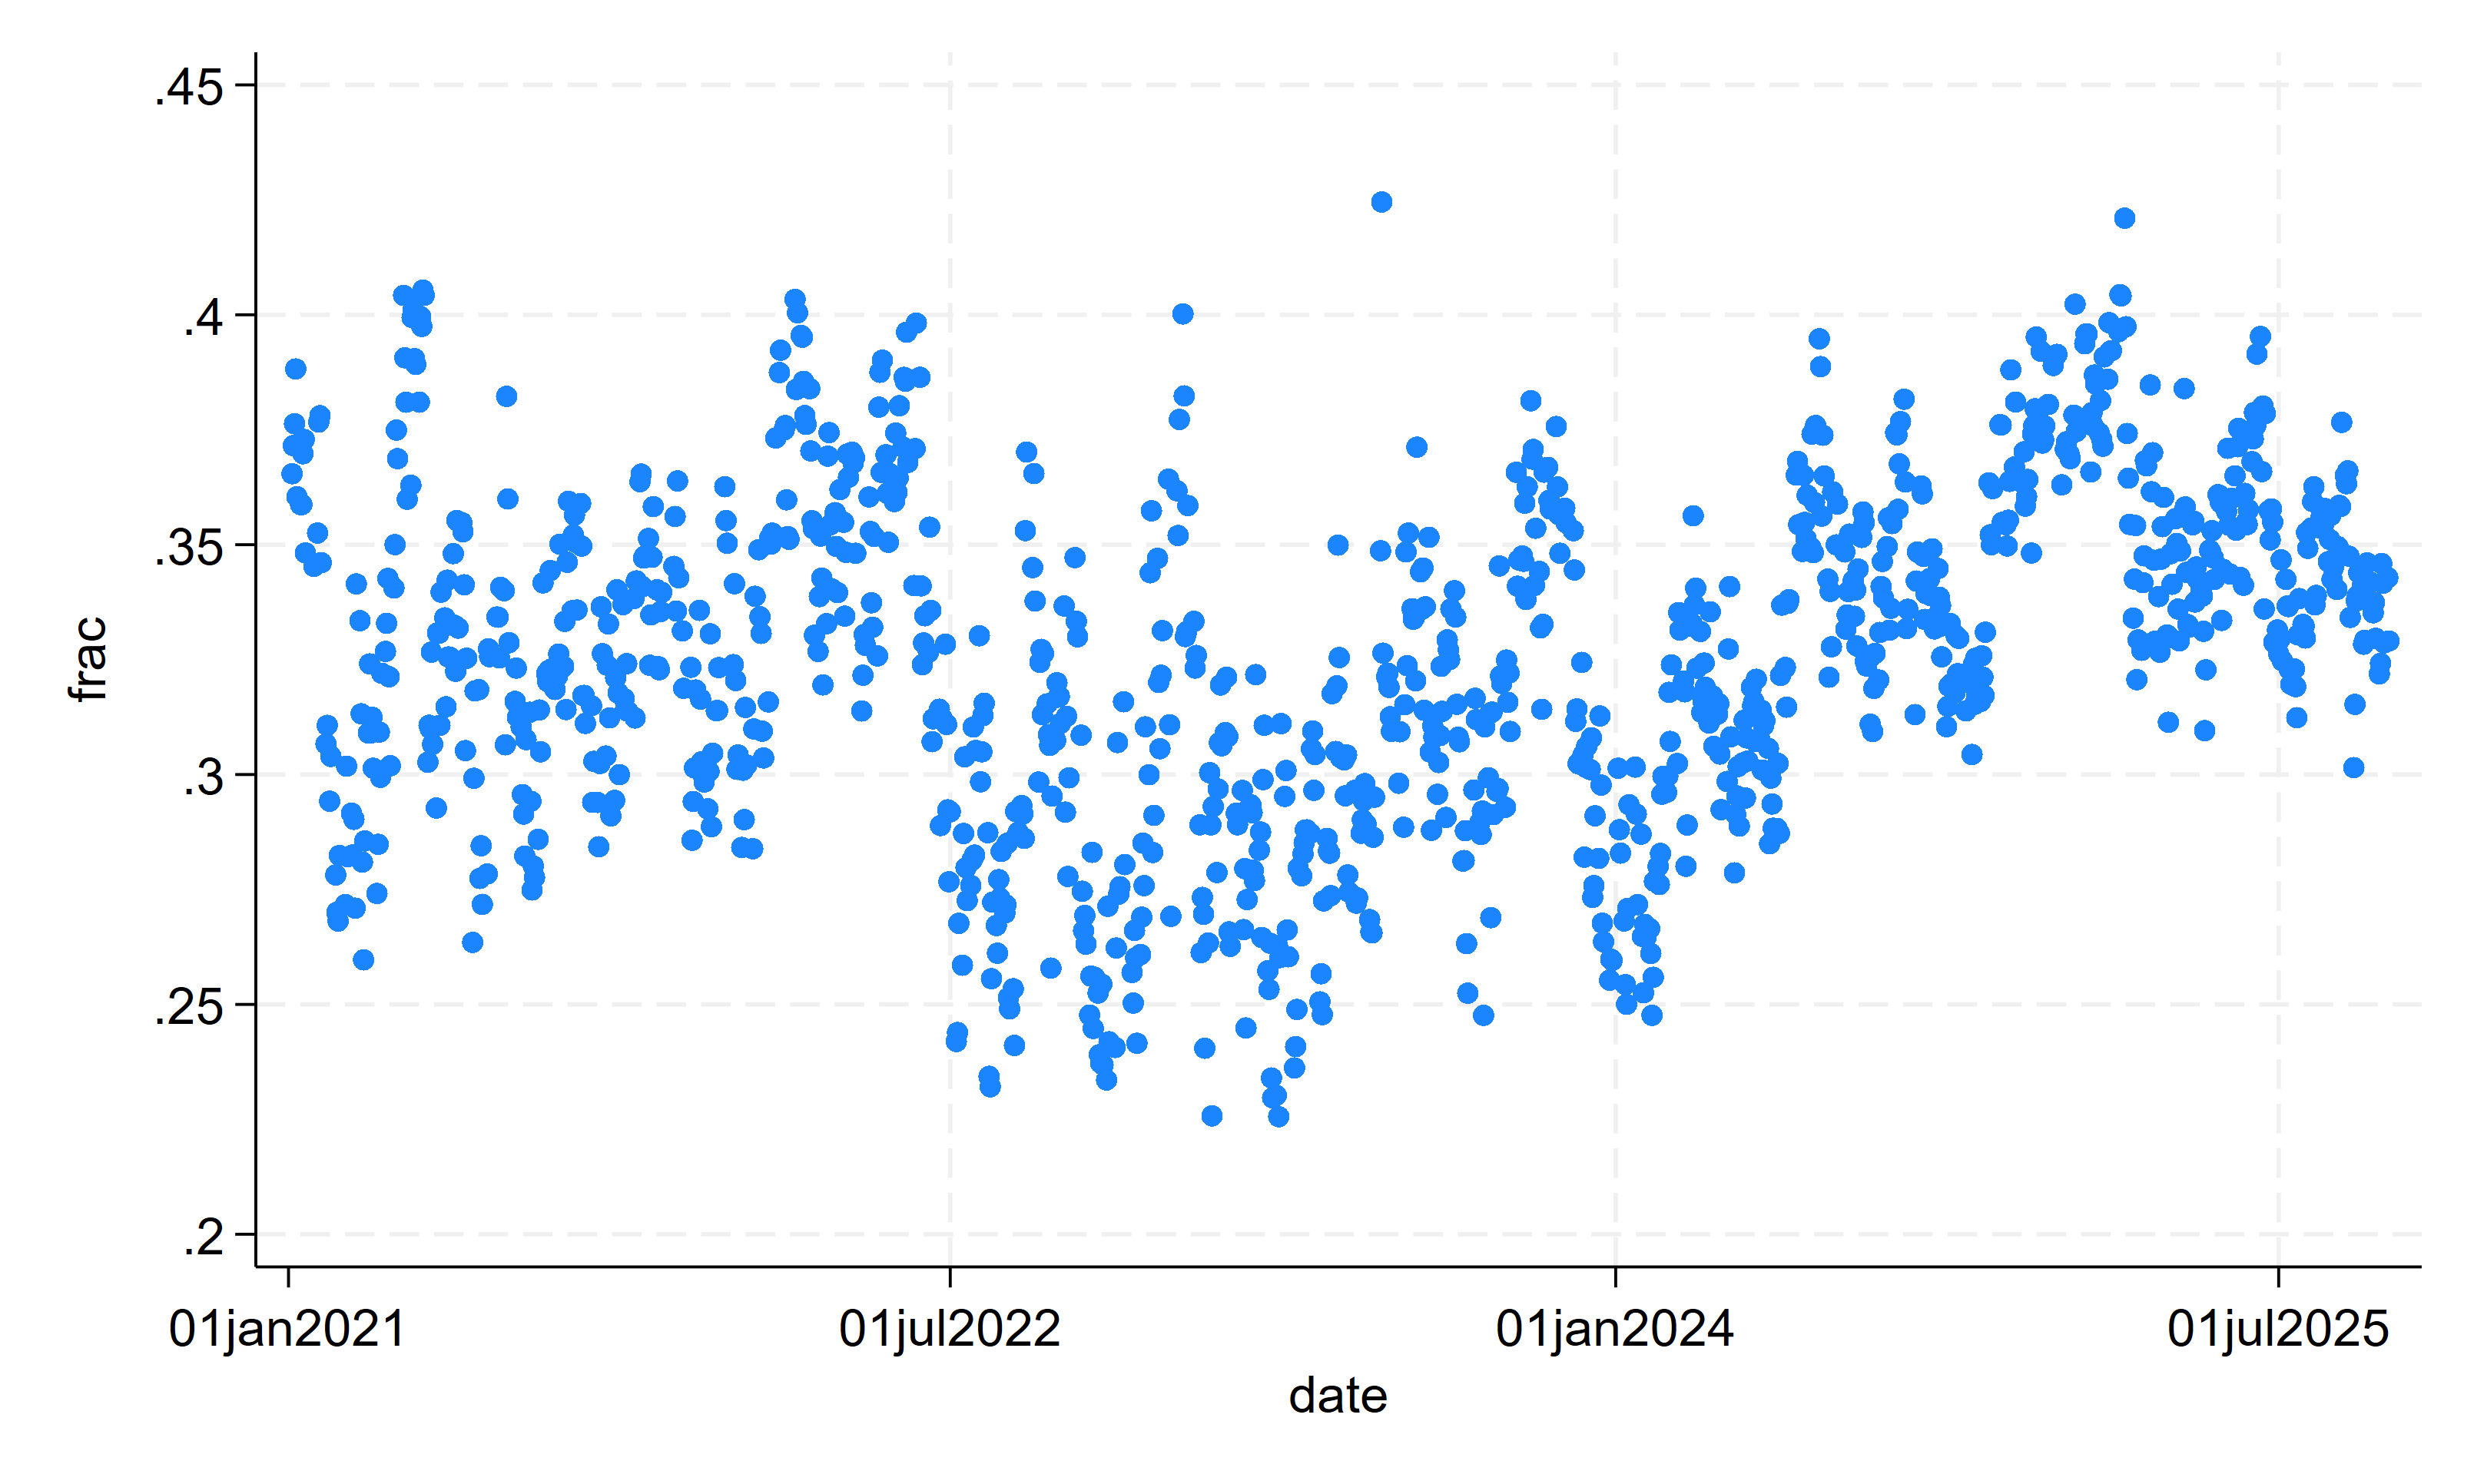
\includegraphics[width=.72\textwidth,height=.68\textheight,keepaspectratio]{frac_top5_funds.png}\\
  {\small\color{slate} Each day the five largest funds are ranked by the absolute value of their net repo position, the chart shows their share in the total across all funds trading directly}
\end{frame}


\begin{frame}{Anatomy of the trade}{Five dealers finance more than half of the trade}
  \centering
  \includegraphics[width=.72\textwidth,height=.68\textheight,keepaspectratio]{Figures/frac_top5_dealers.png}\\
  {\small\color{slate} Each day dealers are ranked by the absolute value of their net EUR repo position with hedge funds, the chart shows the share of the five largest in the total across all dealers}
\end{frame}


\begin{frame}{Anatomy of the trade}{The bonds are not the cheapest to deliver}
  \centering
  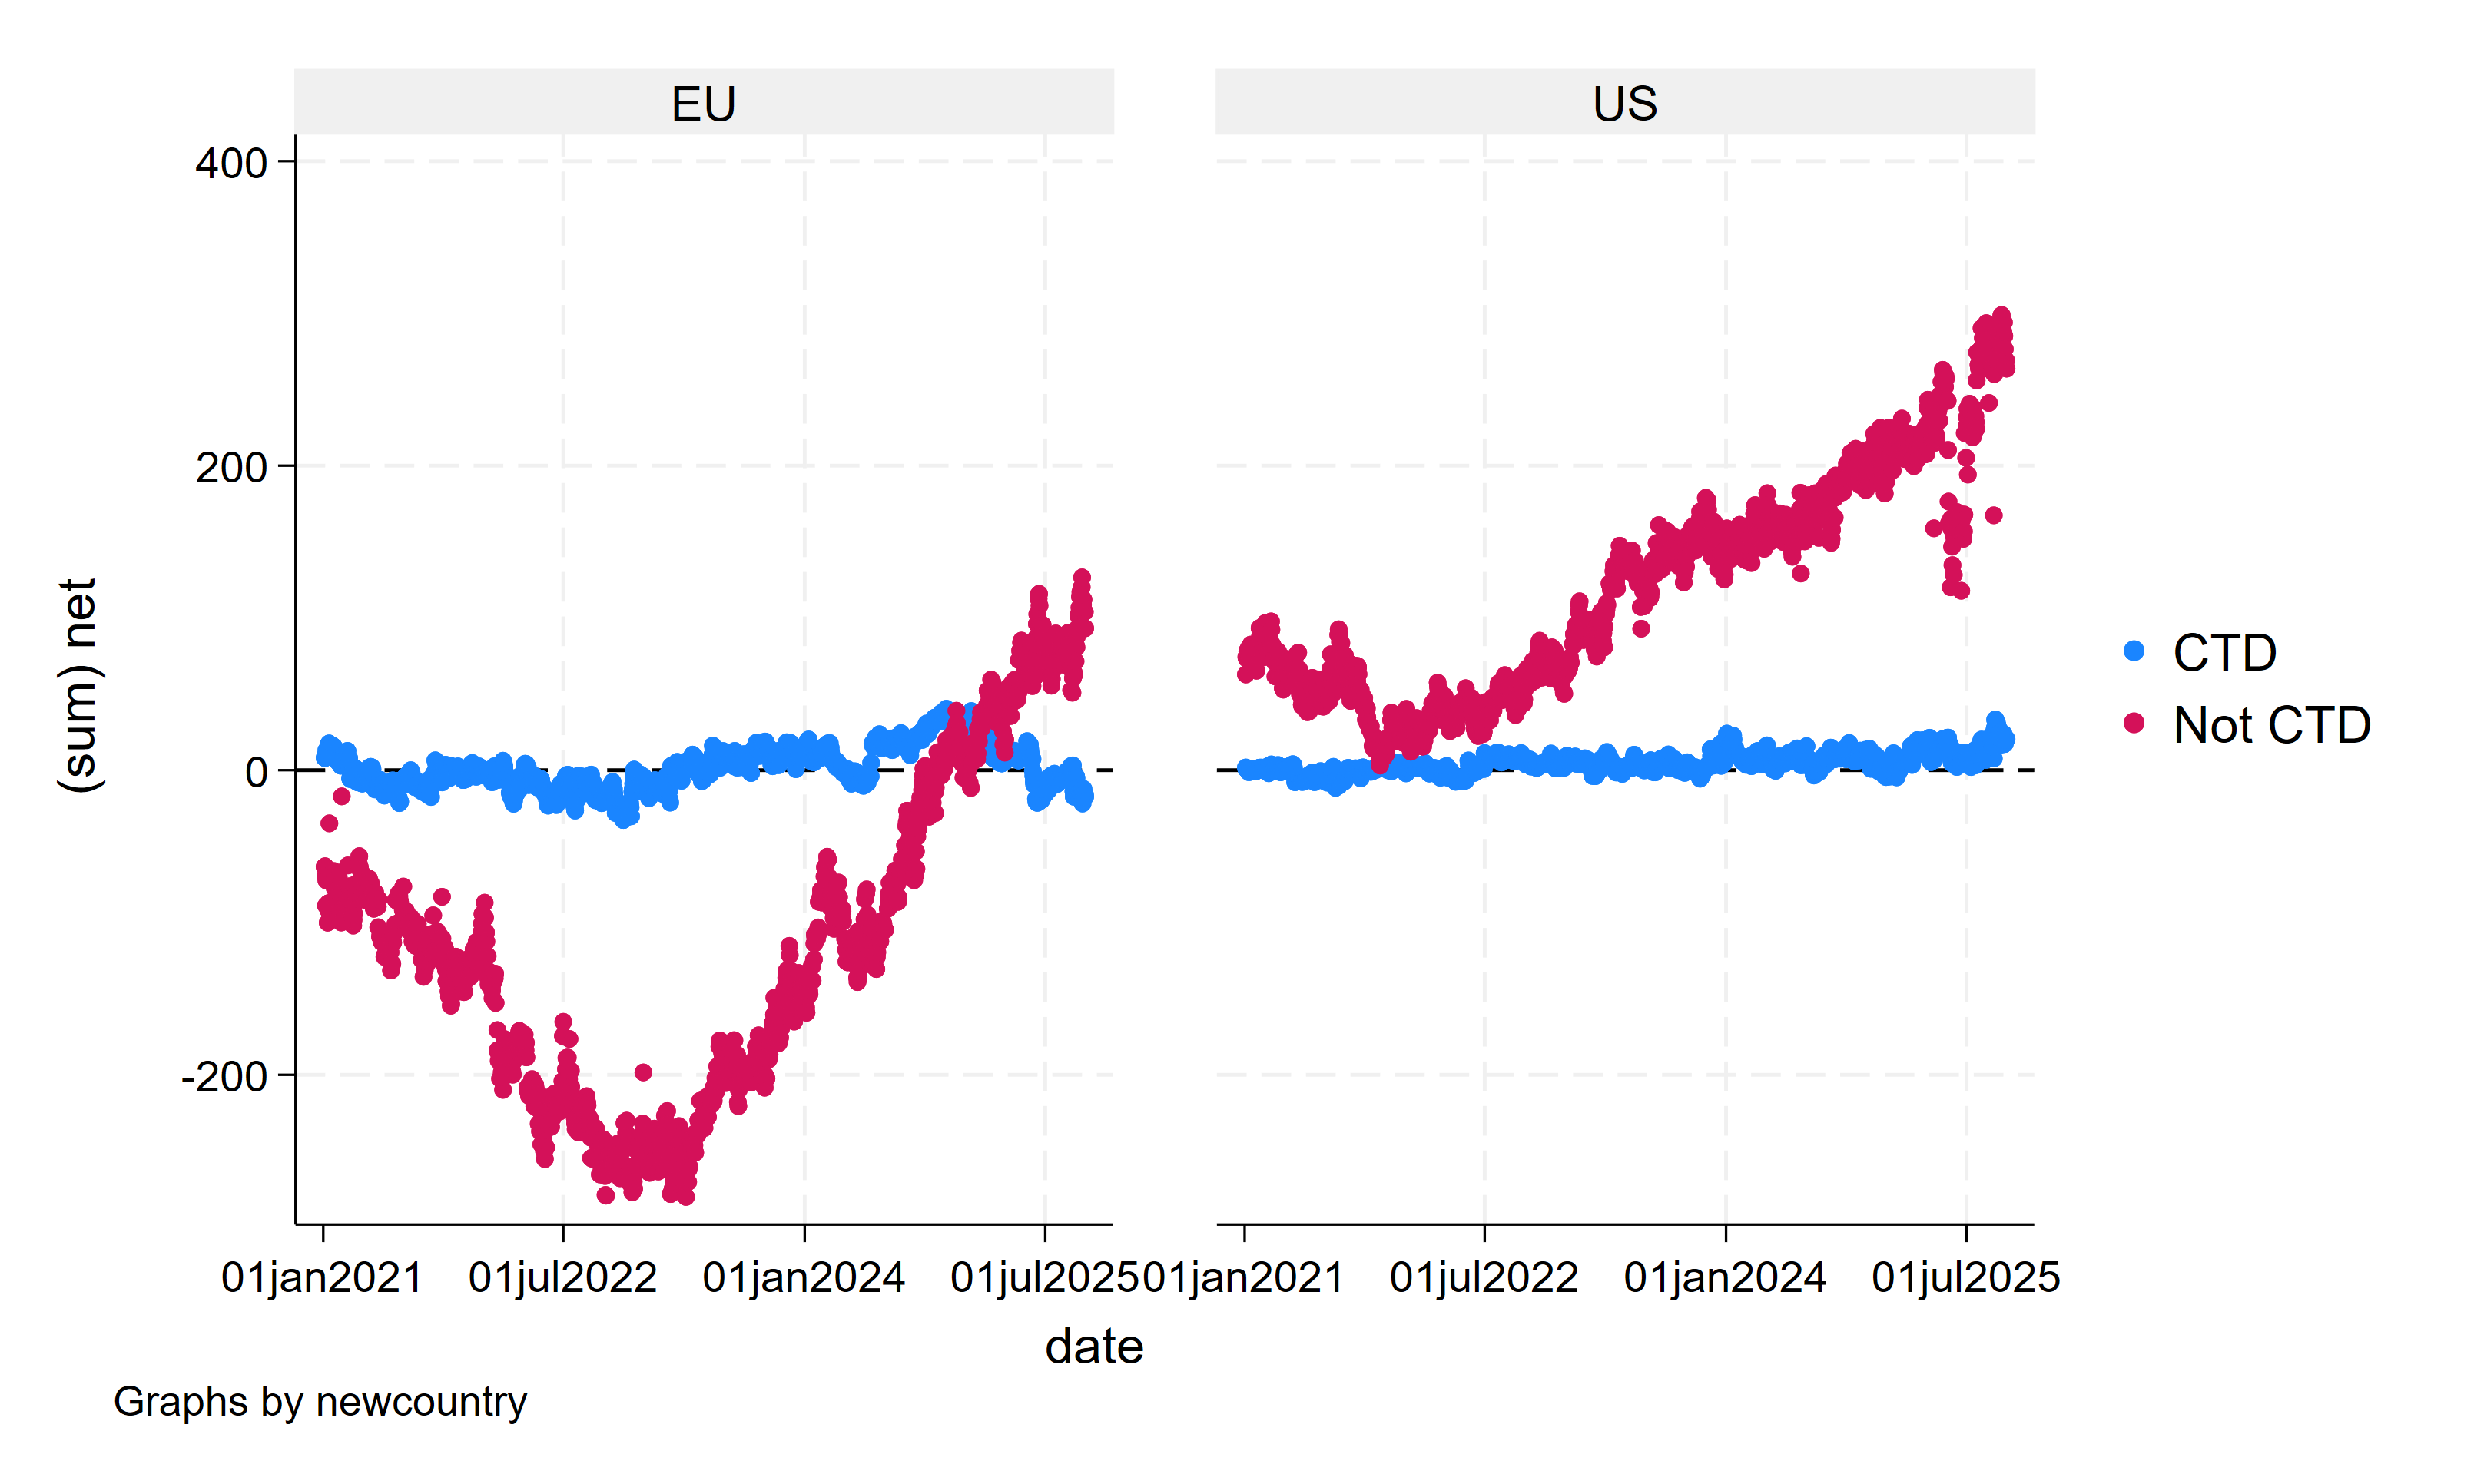
\includegraphics[width=.88\textwidth,height=.7\textheight,keepaspectratio]{ctd.png}\\
  {\small\color{slate} Daily net positions summed across funds, cheapest to deliver bonds against all others}
\end{frame}

\begin{frame}{Anatomy of the trade}{The bonds are not the on the run issues}
  \centering
  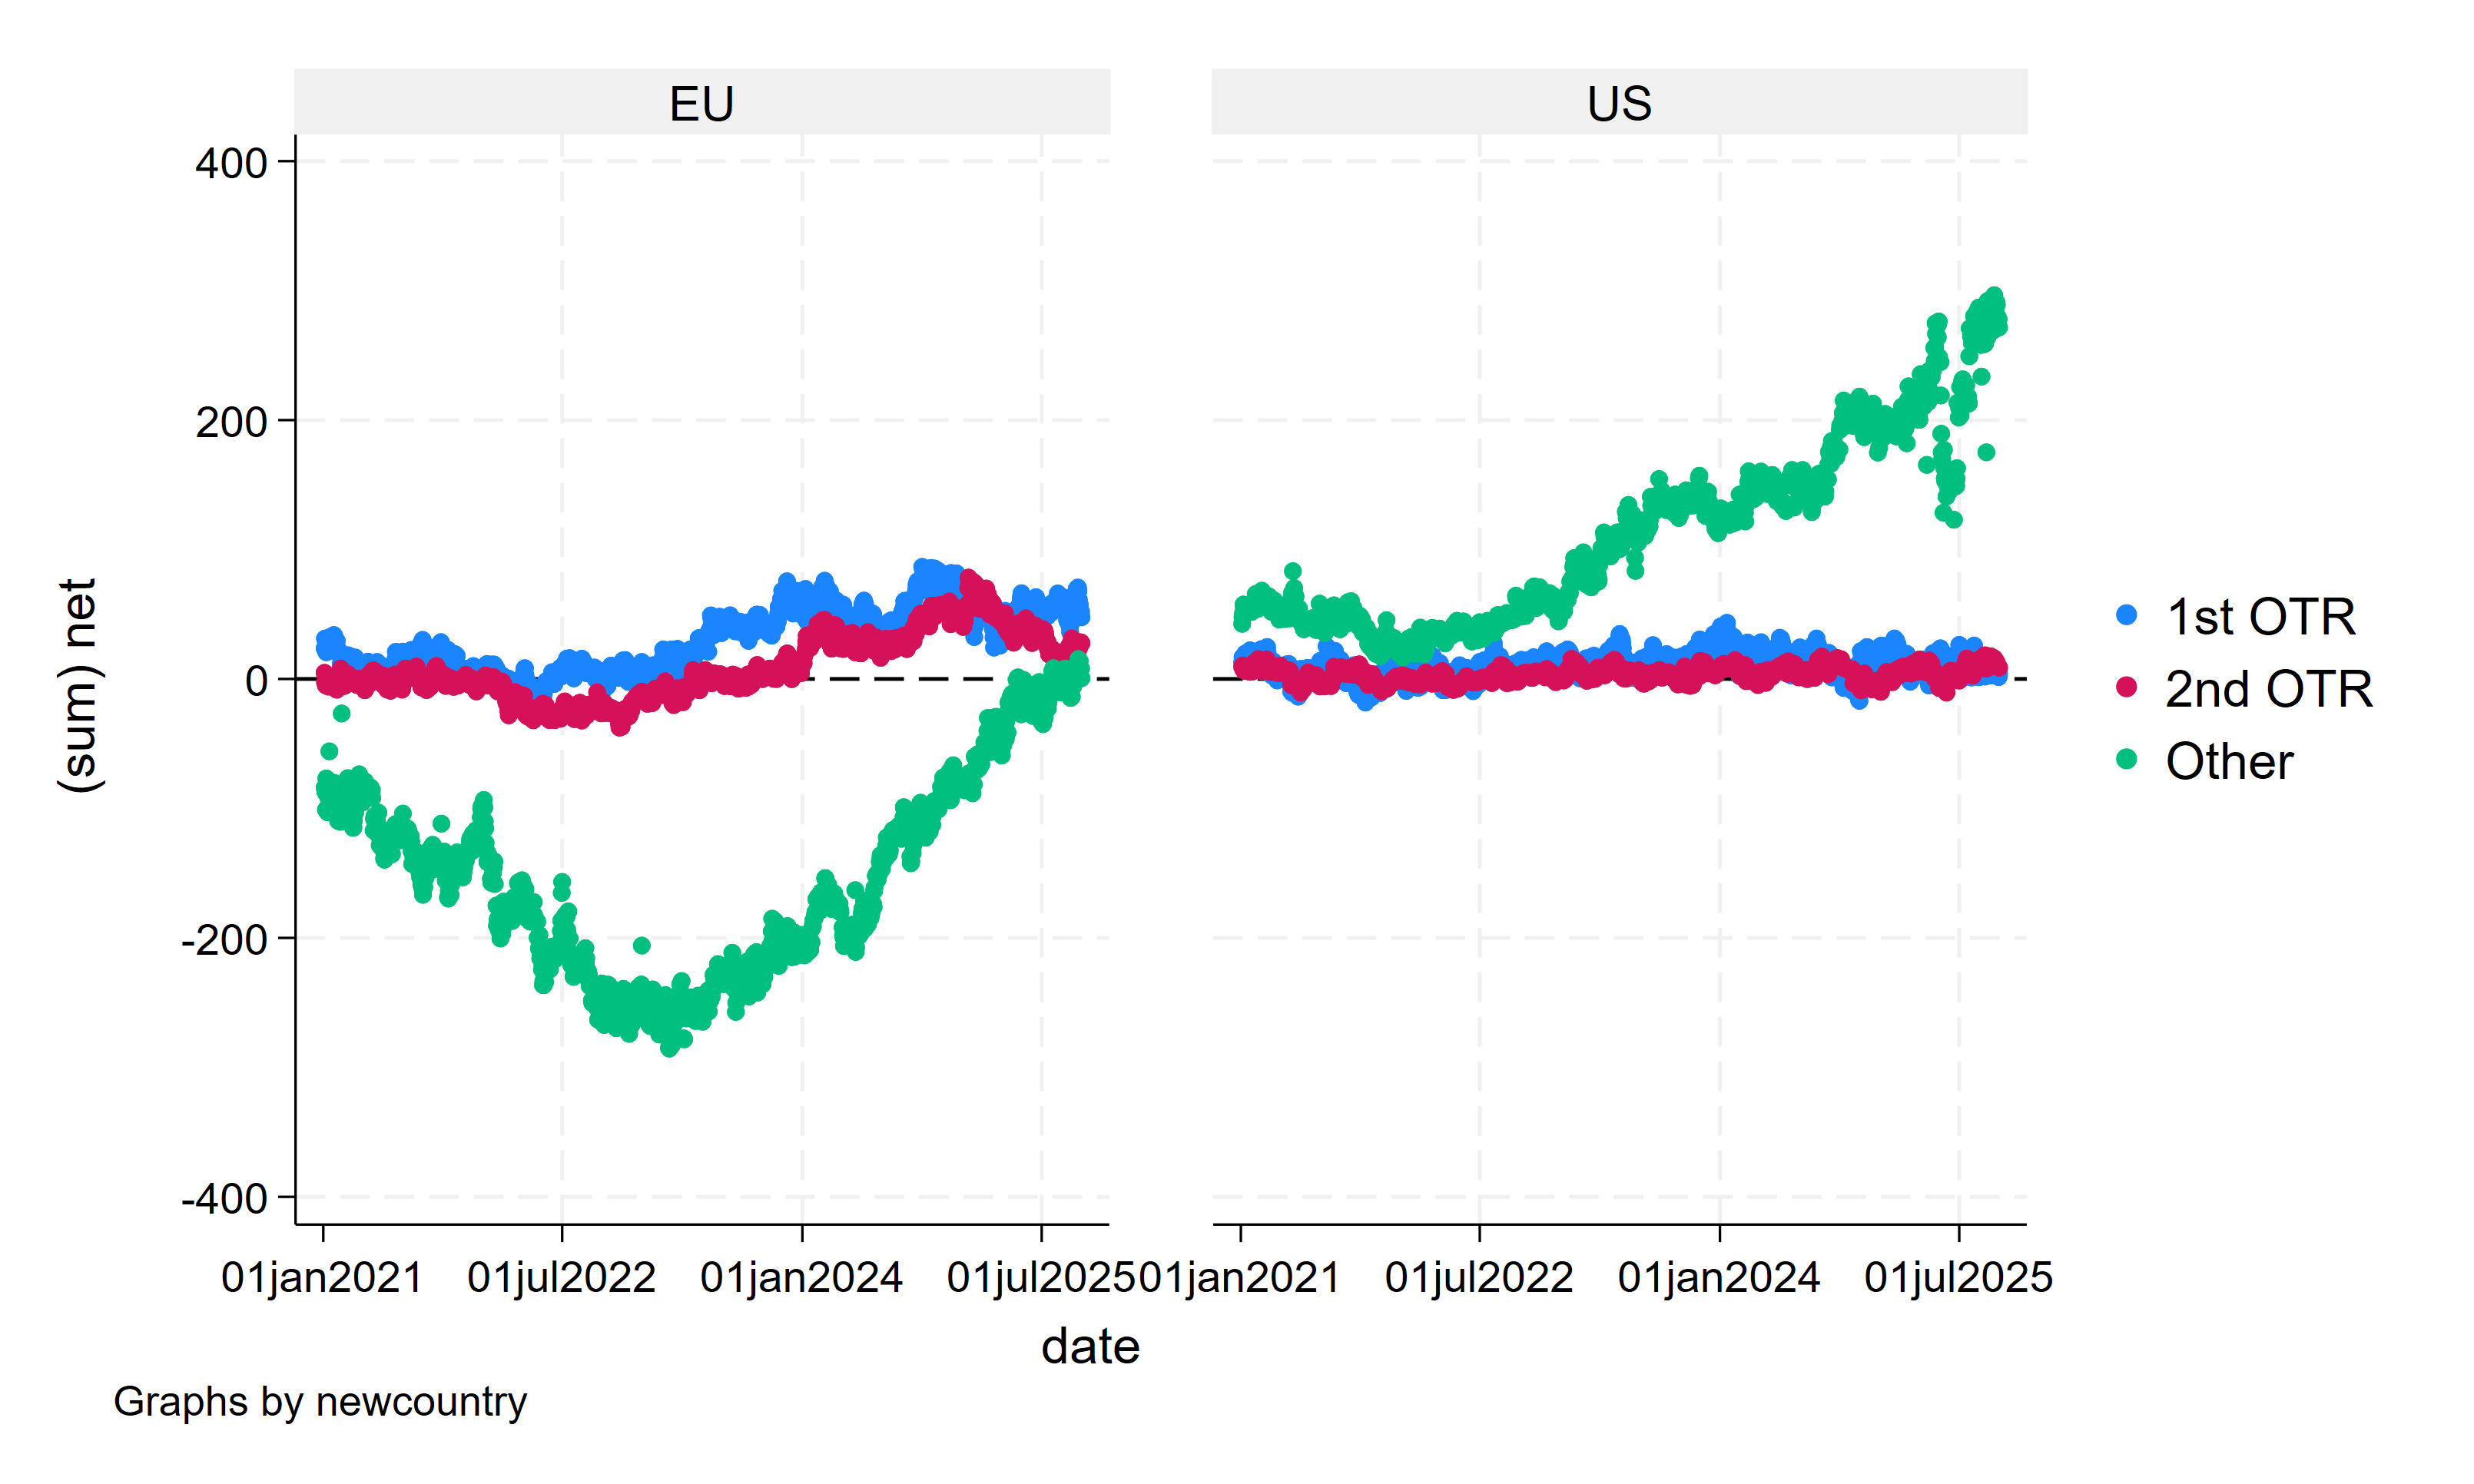
\includegraphics[width=.88\textwidth,height=.7\textheight,keepaspectratio]{otr.png}\\
  {\small\color{slate} Daily net positions summed across funds, first and second on the run issues against all others}
\end{frame}

\begin{frame}{Anatomy of the trade}{Positive Svensson pricing errors}
  \begin{columns}[T]
    \begin{column}{.5\textwidth}\centering
      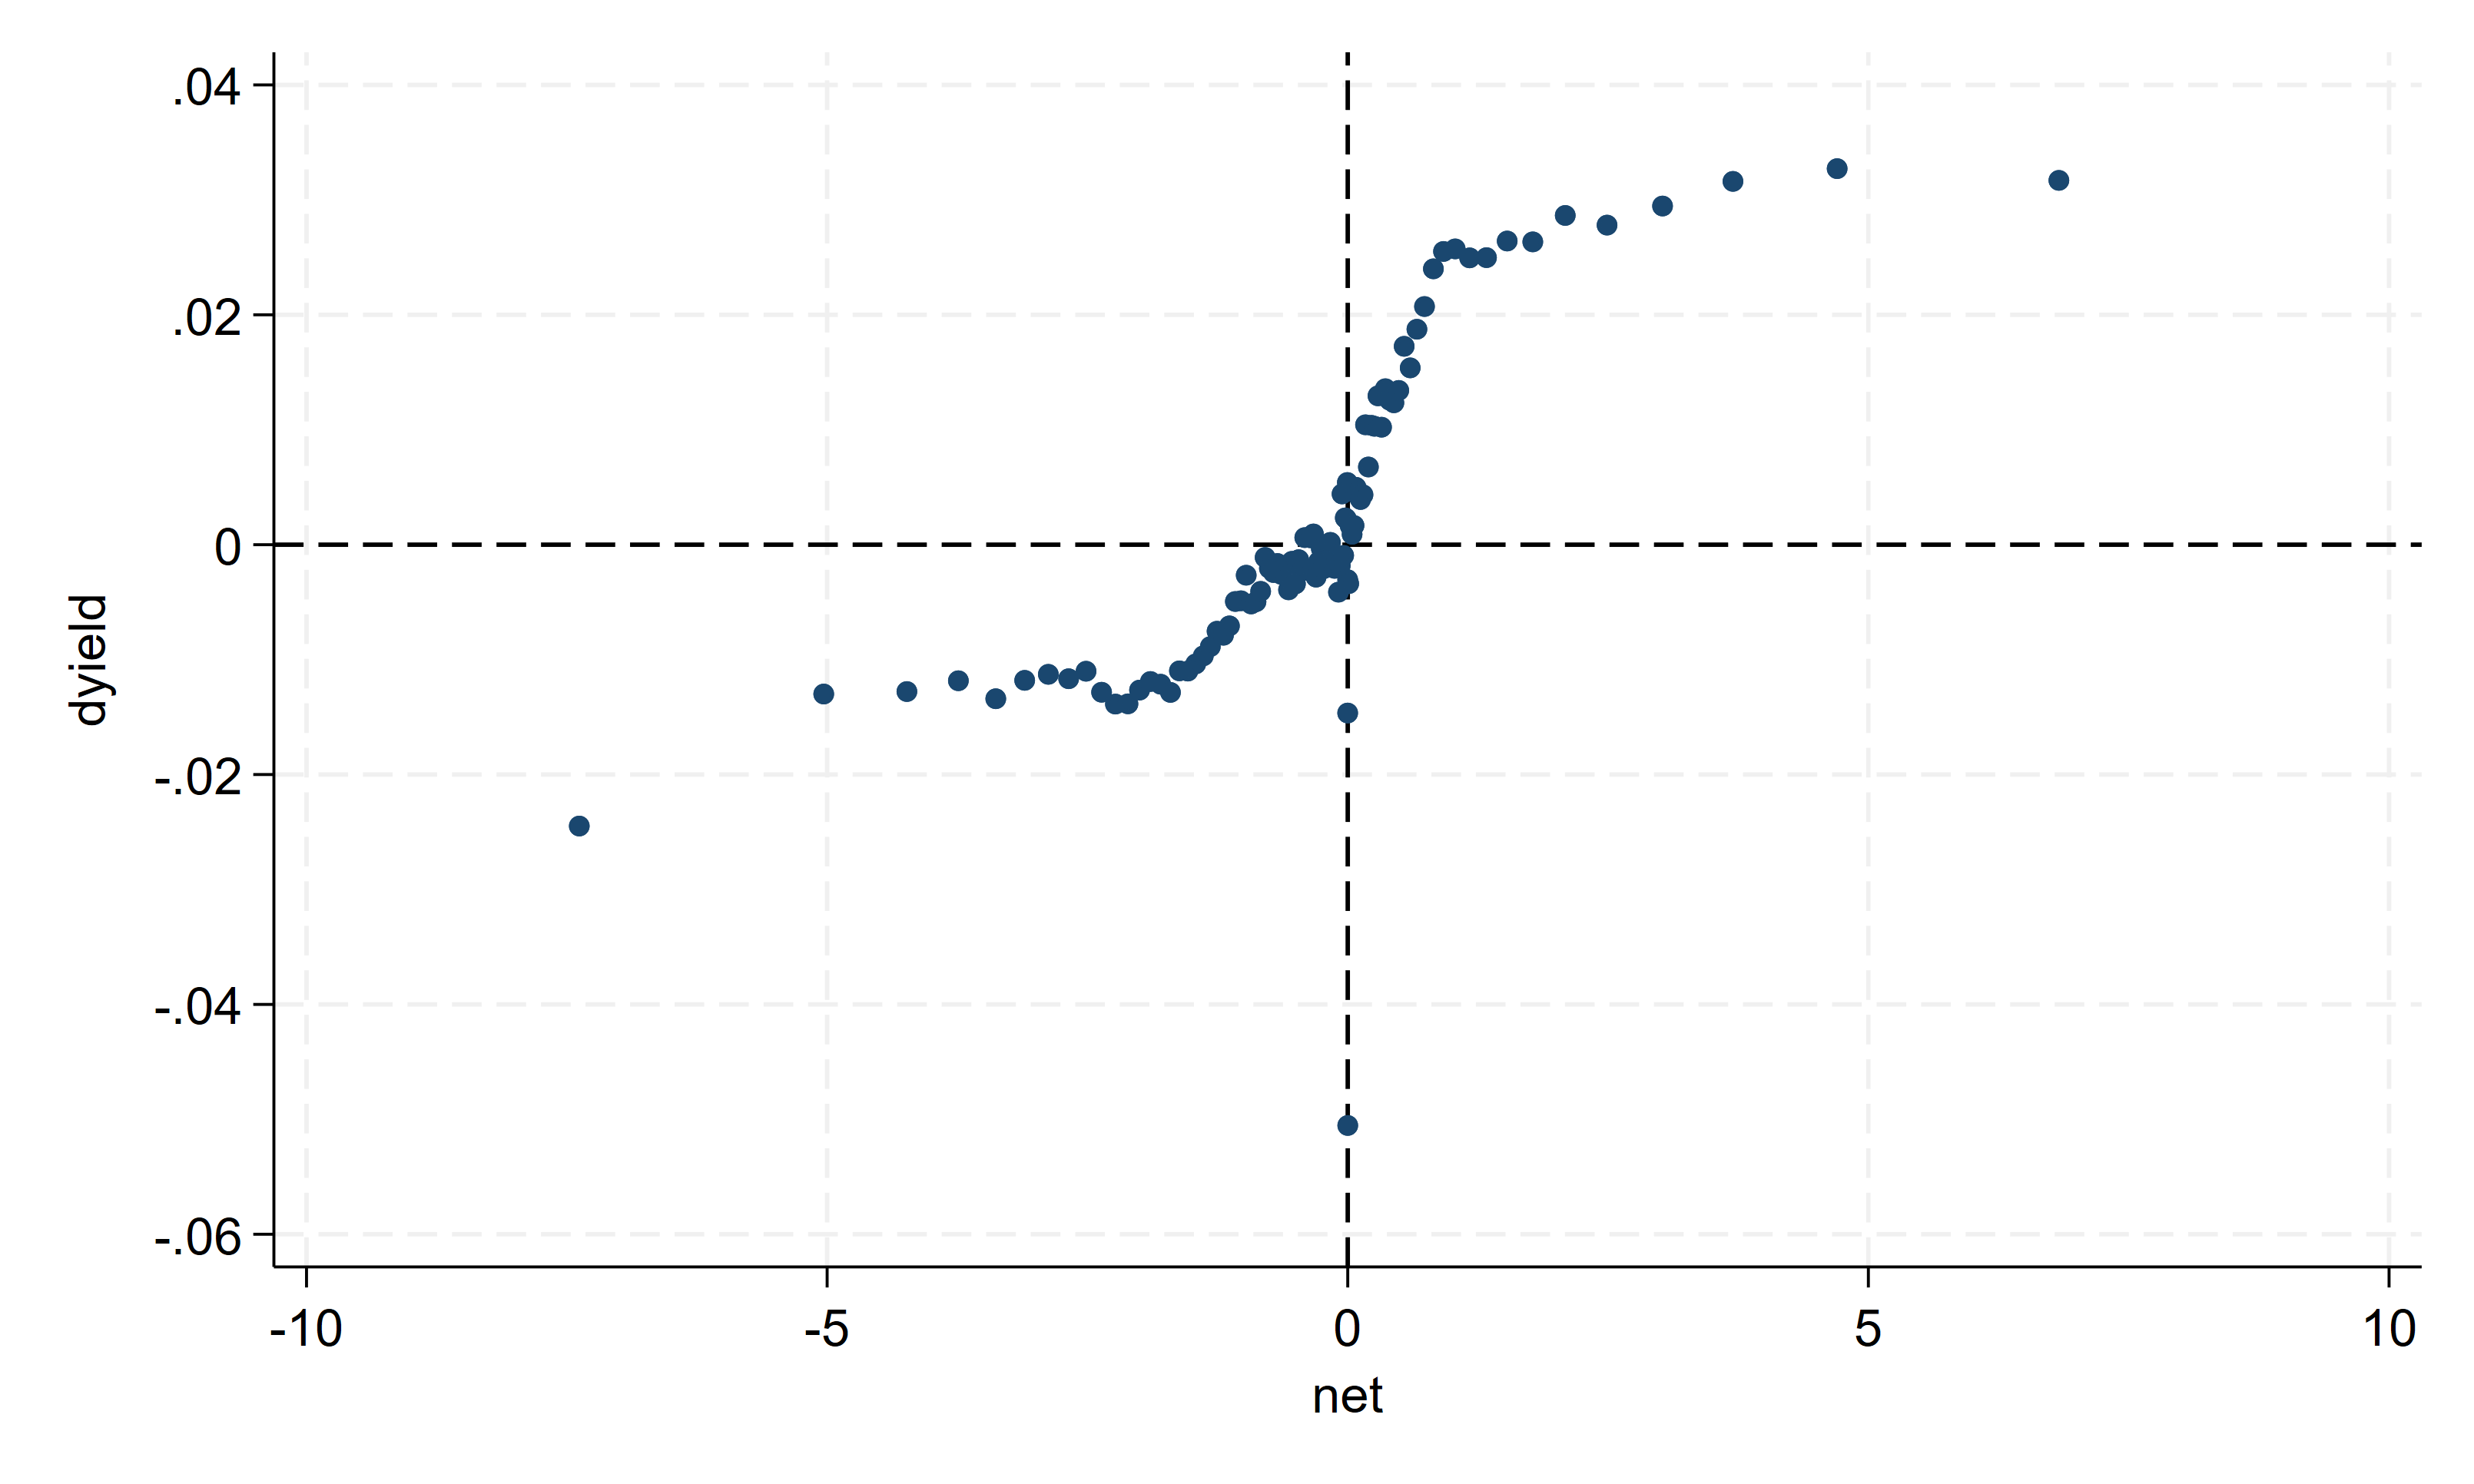
\includegraphics[width=\linewidth,height=.55\textheight,keepaspectratio]{EA_perror.png}\\
      {\small\color{slate} Euro area}
    \end{column}
    \begin{column}{.5\textwidth}\centering
      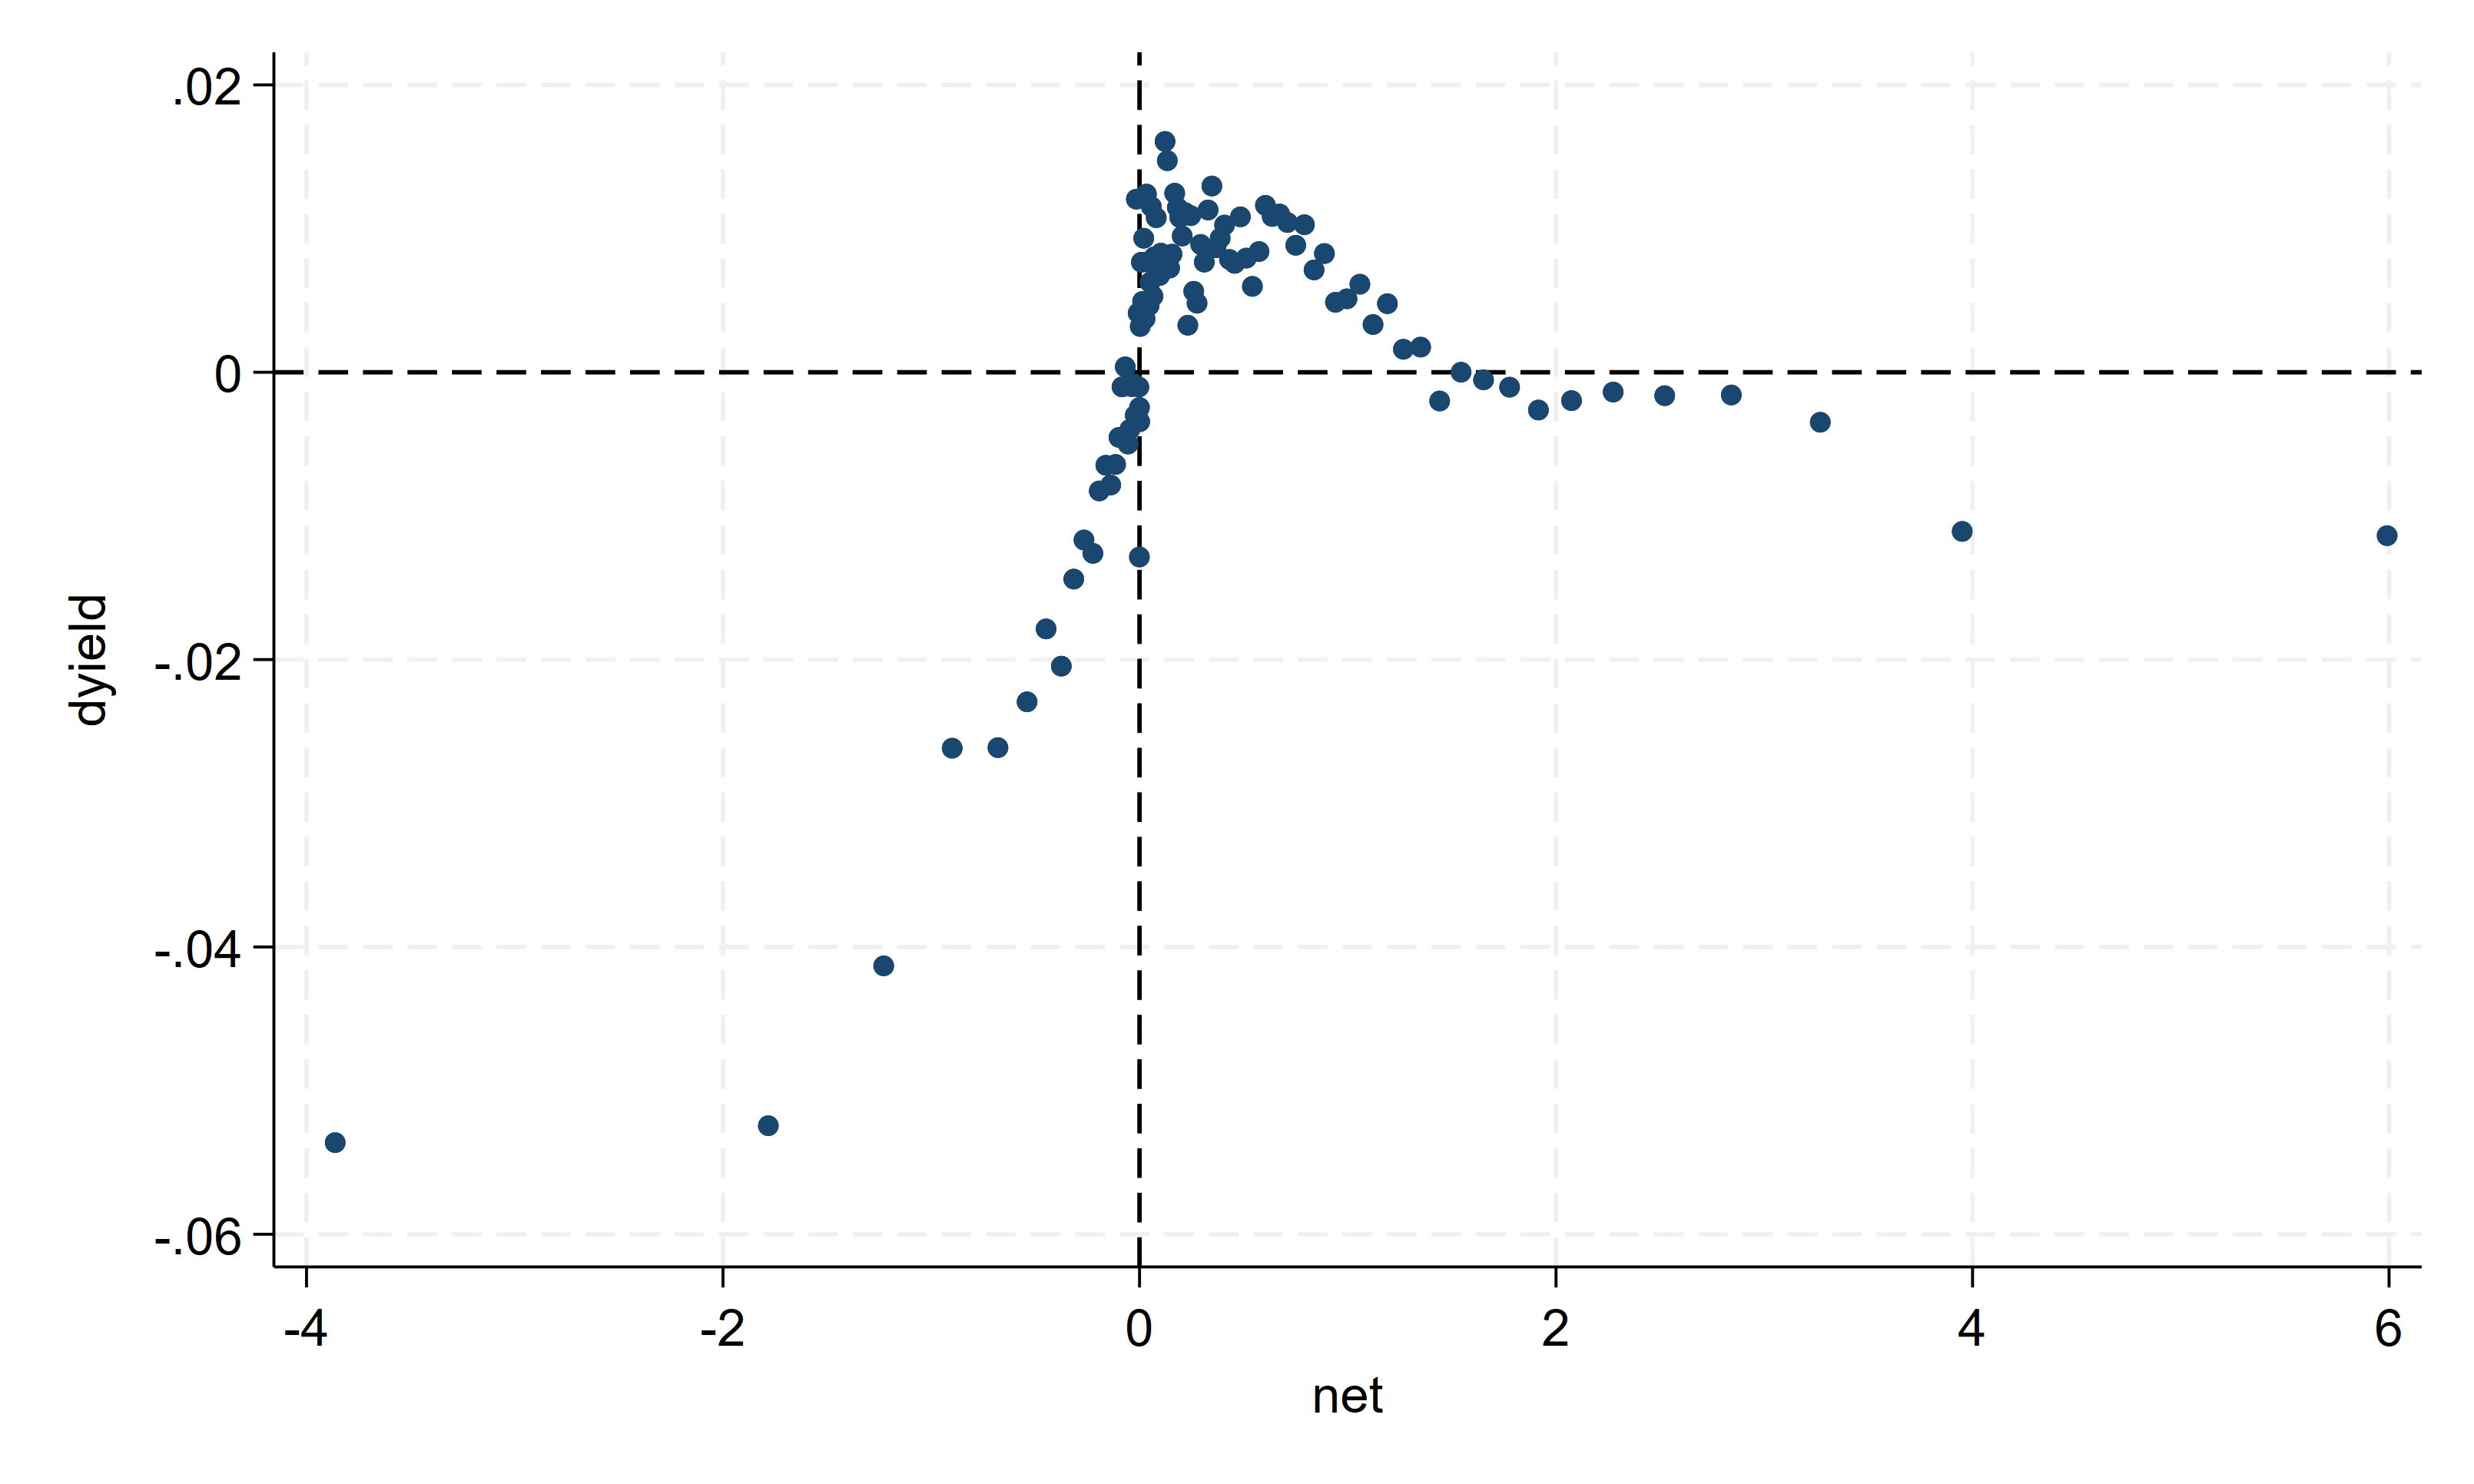
\includegraphics[width=\linewidth,height=.55\textheight,keepaspectratio]{US_perror.png}\\
      {\small\color{slate} US}
    \end{column}
  \end{columns}
  \medskip
  \centering
  {\small\color{slate} Bonds grouped into one hundred bins of net fund positions, each dot shows the bin average deviation of the bond yield from the fitted Svensson curve}
\end{frame}



% ===========================================================================
\section{Risk and return of the trade}
\begin{frame}{Risk and return of the trade}{Duration neutral but convexity exposed}
  \begin{columns}[T]
    \begin{column}{.5\textwidth}\centering
      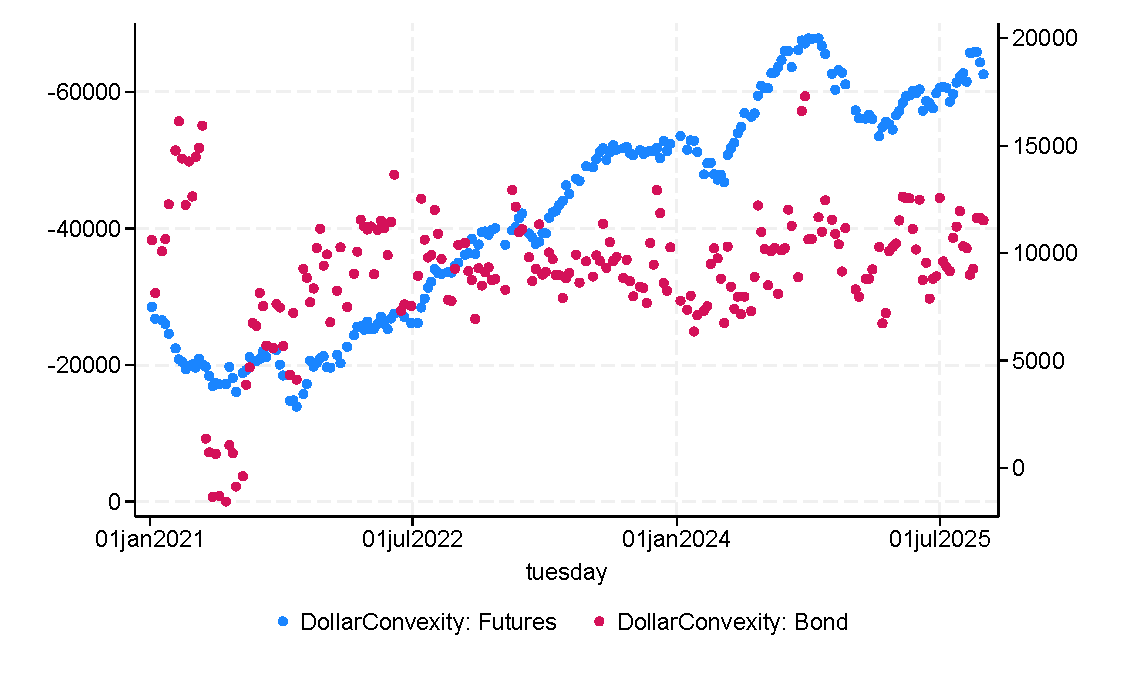
\includegraphics[width=\linewidth,height=.55\textheight,keepaspectratio]{dur1.pdf}\\
      {\small\color{slate} Dollar duration}
    \end{column}
    \begin{column}{.5\textwidth}\centering
      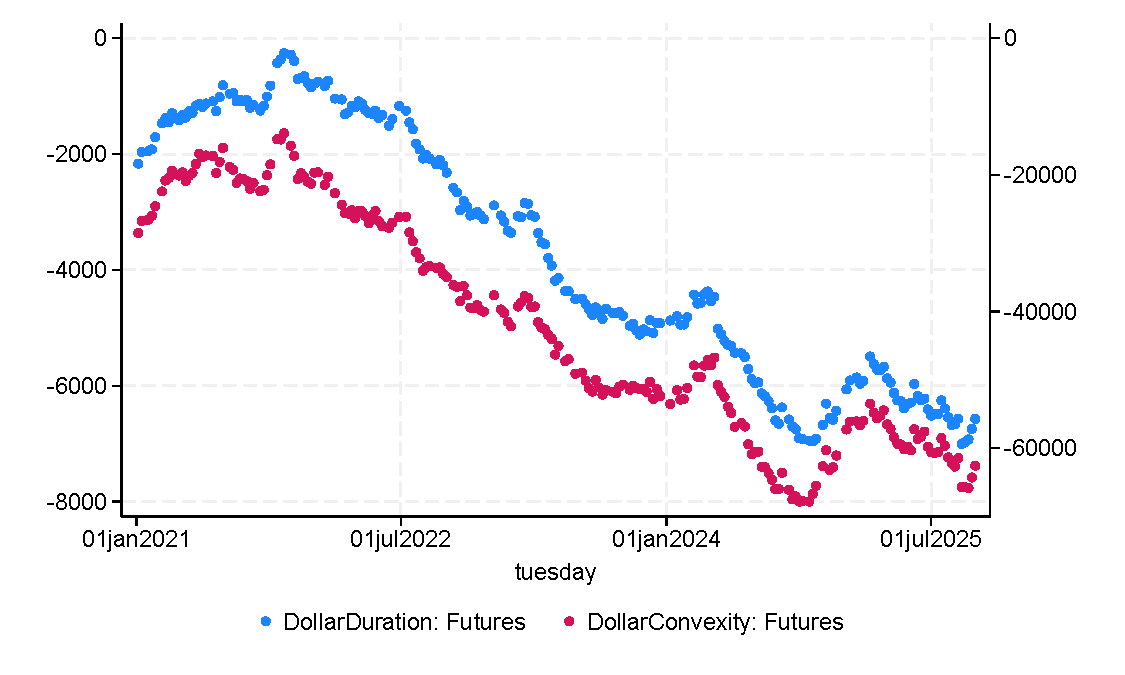
\includegraphics[width=\linewidth,height=.55\textheight,keepaspectratio]{con1.pdf}\\
      {\small\color{slate} Dollar convexity}
    \end{column}
  \end{columns}
  \medskip
  \centering
  {\small\color{slate} US, weekly on Tuesdays. The bond series sums the net repo position times duration or convexity across Treasuries, the futures series does the same across contracts, both in billions. Futures on the left axis, reversed so that offsetting exposures move together, bonds on the right axis}
\end{frame}

\begin{frame}{Risk and return of the trade}{Duration and convexity within each leg}
  \begin{columns}[T]
    \begin{column}{.5\textwidth}\centering
      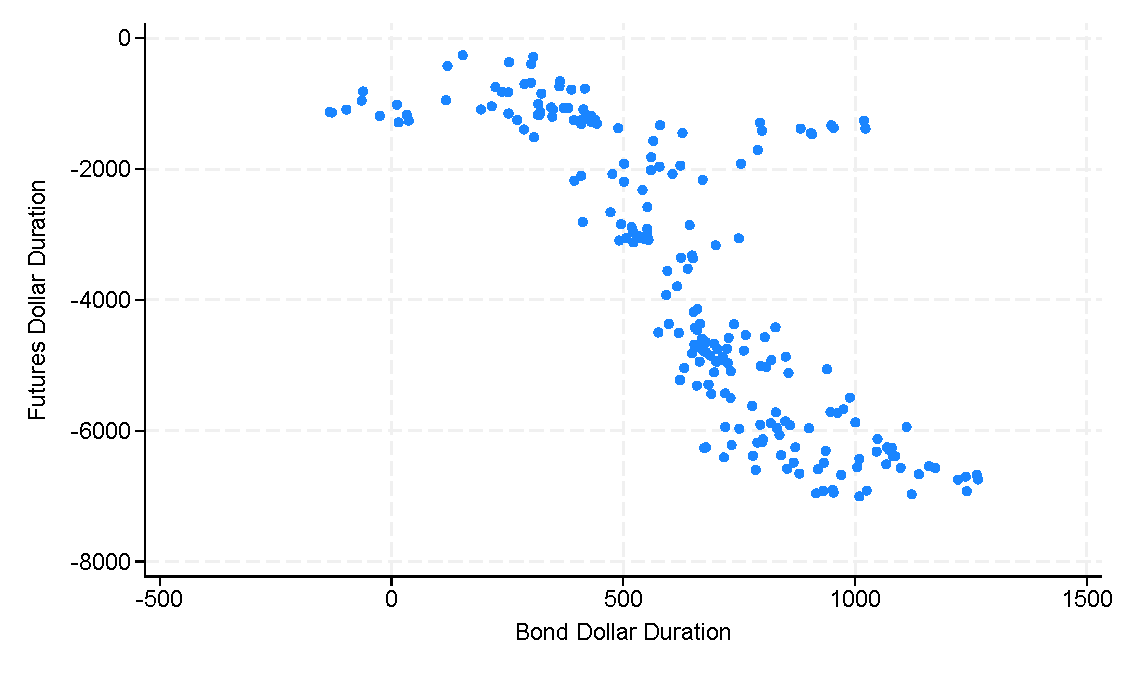
\includegraphics[width=\linewidth,height=.55\textheight,keepaspectratio]{bon1.pdf}\\
      {\small\color{slate} Bonds}
    \end{column}
    \begin{column}{.5\textwidth}\centering
      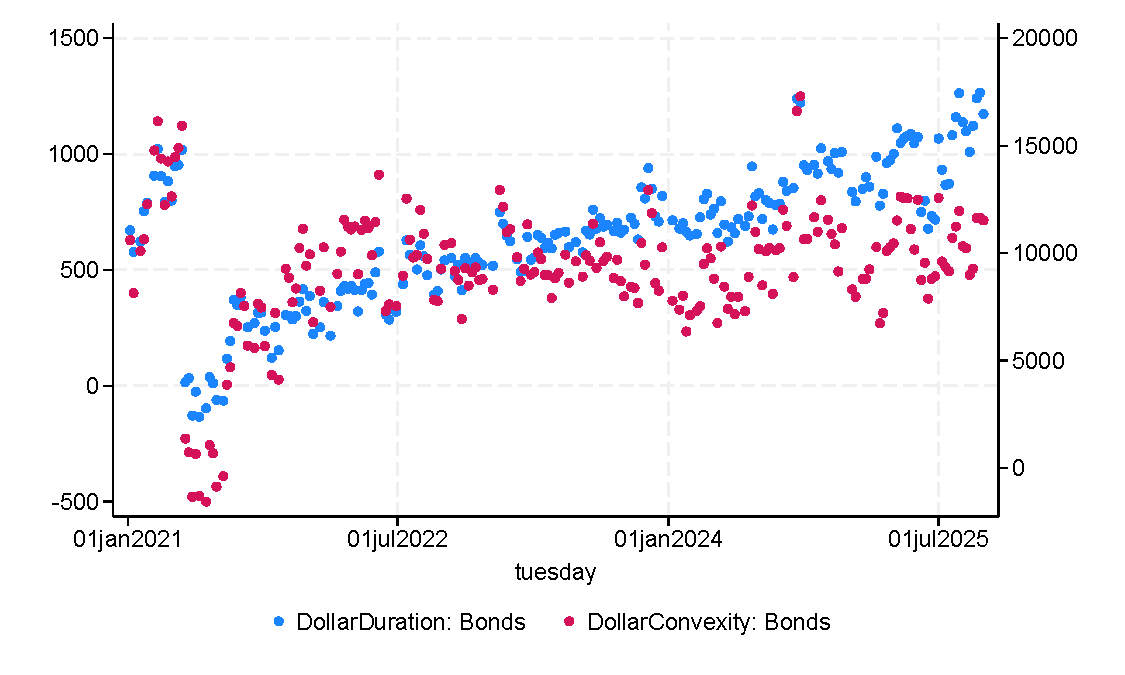
\includegraphics[width=\linewidth,height=.55\textheight,keepaspectratio]{fut1.pdf}\\
      {\small\color{slate} Futures}
    \end{column}
  \end{columns}
  \medskip
  \centering
  {\small\color{slate} Same series as the previous slide, regrouped by leg. Dollar duration on the left axis and dollar convexity on the right axis, US, weekly on Tuesdays, in billions}
\end{frame}

% ===========================================================================
\section{The funding architecture}
\begin{frame}{The funding architecture}{Repo terms by fund dealer pair and relationship stability}
  \vspace{-0.6em}
  \begin{center}\scriptsize
  \begin{tabular}{lrrrr}
    \toprule
    & Mean & p10 & p50 & p90 \\
    \midrule
    \multicolumn{5}{l}{\textit{Fund borrows cash}} \\
    Rate spread to the bond day average (bp) & 5.3 & $-9.6$ & 3.5 & 22.0 \\
    Haircut (percent) & 0.34 & 0.00 & 0.00 & 1.48 \\
    Tenor (days) & 27.1 & 3.5 & 11.7 & 86.0 \\
    \midrule
    \multicolumn{5}{l}{\textit{Fund lends cash}} \\
    Rate spread to the bond day average (bp) & $-4.9$ & $-20.2$ & $-3.7$ & 6.6 \\
    Haircut (percent) & $-0.26$ & $-1.25$ & 0.00 & 0.00 \\
    Tenor (days) & 24.5 & 4.0 & 14.0 & 61.8 \\
    \midrule
    \multicolumn{5}{l}{\textit{Relationships, per fund and quarter}} \\
    Dealers per fund & 2.8 & 1 & 2 & 5 \\
    Share of the largest dealer (percent) & 76 & 41 & 83 & 100 \\
    Share of net position with dealers used a year earlier (percent) & 85 & 41 & 100 & 100 \\
    \bottomrule
  \end{tabular}
  \end{center}
  {\tiny\color{slate} One observation per fund, dealer and day, simple averages over the pair's trades, 301 thousand on the borrowing and 338 thousand on the lending side. The rate spread is the pair's rate minus the average over all other trades in the same bond on the same day, the fund's own trades excluded. Relationships use absolute net positions over 3,201 fund quarters.\par}
\end{frame}



\end{document}